\documentclass{report}
\usepackage[T1]{fontenc} % Fontes T1
\usepackage[utf8]{inputenc} % Input UTF8
\usepackage[backend=biber, style=ieee]{biblatex} % para usar bibliografia
\usepackage{csquotes}
\usepackage[portuguese]{babel} %Usar língua portuguesa
\usepackage{blindtext} % Gerar texto automaticamente
\usepackage{hyperref} % para autoref
\usepackage{graphicx}
\usepackage{indentfirst}
\usepackage[printonlyused]{acronym}


\bibliography{bibliografia}


\begin{document}
%%
% Definições
%
\def\titulo{CIBERSEGURANÇA}
\def\data{DATA}
\def\autores{Rúben Gomes, Tiago Garcia}
\def\autorescontactos{113435 rlcg@ua.pt, 114184 tiago.rgarcia@ua.pt}
\def\versao{VERSÃO 1}
\def\departamento{Dept. de Eletrónica, Telecomunicações e Informática}
\def\empresa{Universidade de Aveiro}
\def\logotipo{ua.pdf}

%
%%%%%% CAPA %%%%%%
%
\begin{titlepage}

\begin{center}
%
\vspace*{50mm}
%
{\Huge \titulo}\\ 
%
\vspace{10mm}
%
{\Large \empresa}\\
%
\vspace{10mm}
%
{\LARGE \autores}\\ 
%
\vspace{30mm}
%
\begin{figure}[h]
    \center
    
\includegraphics{ua}
\end{figure}
%
\vspace{30mm}
\end{center}
%
\begin{flushright}
\versao
\end{flushright}
\end{titlepage}

%%  Página de Título %%
\title{%
{\Huge\textbf{\titulo}}\\
{\Large \departamento\\ \empresa}
}
%
\author{%
    \autores \\
    \autorescontactos
}
%
\date{\today}
%
\maketitle

\pagenumbering{roman}

%%%%%% RESUMO %%%%%%
\begin{abstract}
Neste trabalho é abordado o tema de cibersegurança, tema este que, com desenvolver gradual das tecnologias, torna-se cada vez mais importante. \ Vulnerabilidades surgem a cada dia, e há cada vez mais ataques cibernéticos. \ Com este projeto procuramos tocar nos pontos mais importantes do mundo digital. \bigskip

Este trabalho está dividido em 2 grandes capítulos, a Cibersegurança no geral e as Vulnerabilidades. \par
O capítulo da Cibersegurança no geral fala de uma ideia geral da cibersegurança, a sua importância, os tipos de ameaças existentes, como ataques, botnets, malware, entre muitos outros. \ O grande objetivo deste capítulo é introduzir ao leitor o conceito de cibersegurança, o que é, para que é importante bem como os diversos perigos a que o usuário comum está exposto nos dias que correm. \par
O capítulo das Vulnerabilidades fala, como o nome indica, de vulnerabilidades em sistemas. \ Entre os métodos de análise, definições de termos usados em cibersegurança, e programas utilizados para o combate às mesmas, procura-se demonstrar ao leitor o quão vasto é o mundo online, e que o mundo todo está constantemente exposto a vários tipos de vulnerabilidades. \ Embora acabem por existir soluções, cada um deve ter sempre o seu cuidado a usar uma máquina. \ É também importante reforçar a ideia que o software usado em análises é permutável, ou seja, ao usá-lo mutuamente, obtém-se melhores resultados(desde que não tenham os mesmos propósitos!). \bigskip

Com isto, os autores consideram que este relatório é ideal para qualquer leitor que deseja saber algo mais sobre o mundo digital.
\end{abstract}

%%%%%% Agradecimentos %%%%%%
%Segundo glisc deveria aparecer após conclusão
%\renewcommand{\abstractname}{Agradecimentos}
%\begin{abstract}
%Eventuais agradecimentos.
%Comentar bloco caso não existam agradecimentos a fazer.
%\end{abstract}


\tableofcontents
\listoftables     % descomentar se necessário
\listoffigures    % descomentar se necessário


%%%%%%%%%%%%%%%%%%%%%%%%%%%%%%%
\clearpage
\pagenumbering{arabic}

%%%%%%%%%%%%%%%%%%%%%%%%%%%%%%%%
\chapter*{Introdução}
\label{ch:introducao}

Com o passar dos anos, as tecnologias que temos ao nosso dispor tem evoluído de uma forma rápida e sem fim, como, por exemplo, o \textit{hardware} de um computador.\ Mas, com constantes evoluções, também vem uma necessidade de responsabilidade, pois com quanto mais recursos existirem, maior será o impacto de danos a indivíduos ou entidades.\\

Com este relatório, irá ser abordado um tópico bastante sensível na atualidade, a Cibersegurança, bem como as diversas vulnerabilidades associadas de formas de nos protegermos contra as mesmas.

\chapter{Cibersegurança no geral}
\label{ch:ciberseguranca-no-geral}
\section{Conceito}
Quando os sistemas e ambientes digitais foram criados não existia quase nenhuma interação entre dispositivos e a pouca que existia era efetuada por cabo.\ Porém, quando a internet foi criada, a interação entra dispositivos digitais aumentou e com isso, tal como acontece com interações humanas, vieram diversos perigos e ameaças aos utilizadores.\ Da mesma forma que existem crimes no mundo físico também existem crimes digitais e da mesma forma que existem soluções e entidades responsáveis pela prevenção e combate a crimes físicos, também os mesmos existem para o mundo digital, proporcionando cibersegurança aos utilizadores da internet e ambientes digitais.

\section{Tipos de ameaças}
\subsection{Ameaças cibernéticas}
Conjunto de malware e software com capacidade de afetar o funcionamento normal de equipamentos digitais.\ Muitas vezes usadas para ciberterrorismo e causar danos graves com o intuito de lucrar ou impossibilitar o trabalho usual de uma entidade.\\
\subsubsection{\large Botnets}
\label{subsubsec:botnets}
Botnets são robos digitais que conseguem infetar dispositivos, tal como um vírus e a partir daí permitir que utilizadores remotos tenham acesso à máquina onde se encontram alojados.\ Estas máquinas são muitas vezes usadas para fazer tarefas ilícitas e ilegais por parte do utilizador remoto sem que este seja exposto por não ser a máquina do mesmo a realizar as ações.
\par Estes botnets podem contaminar computadores, dispositivos móveis, \textit{routers} e dispositivos \ac{iot}.
\par Da mesma maneira que um vírus tenta infetar o corpo humano através de falhas no sistema imunitário, também estes bots tentam infetar os dispositivos através de falhas de segurança.\ É possível detetar que o dispositivo se encontra infetado a partir da deteção de comportamentos anormais por parte da máquina, por exemplo quando esta trabalha de forma mais lenta do que o normal ou quando durante a utilização aparecem mensagens de erro aleatórias.\\
\subsubsection{Tipos de botnets}
Dentro dos botnets existem dois tipos: \underline{Cliente Servidor} e \underline{Peer-to-Peer}

\begin{itemize}
\item Cliente servidor $\rightarrow$
Este é o modelo dos botnets mais antigos em que os dispositivos infetados (clientes) recebem intruções de um outro dispositivo que os controla (servidor)
\item Peer-to-peer $\rightarrow$ Este modelo corrige algumas falhas que o modelo de cliente servidor tinha.\ Em vez de ser establecida apenas uma conexão entre dois dispositivos (cliente e servidor), neste modelo todos os dispositivos infetados estão conectados entre si, todos a ser controlados pelo mesmo dispositivo que dá as intruções a todos os outros.\ Isto permite que no caso de haver uma falha com um dos dispositivos infetados, a rede continue online e funcional.\\
\end{itemize}
\subsubsection{\large \ac{ddos}}
\label{subsubsec:ddos}
Estas ameaças são das mais comuns e mais utilizadas pela comunidade de atacantes.\ O objetivo destes ataques é levar o consumo de recursos do servidor/aplicação ao limite.\ Uma vez sem recursos disponiveis, o servidor acaba por ter falhas de funcionalidade ou pode chegar mesmo a ir abaixo e ficar offline.\\
A quantidade dste tipo de ataques têm vindo a aumentar substancialmente, segundo a Microsoft\footnote{Fonte: \url{https://www.microsoft.com/en-us/security/business/security-101/what-is-a-ddos-attack}}, a Azure Networking registou, em 2021, um aumento de 25\% a mais de casos de \ac{ddos} em relação a 2020.

\subsubsection{Functionamento de \ac{ddos}}
Durante estes ataques, um conjunto de Botnets~(\ref{subsubsec:botnets}) ataca uma aplicação/servidor com o objetivo de desgastar e levar o consumo de recursos ao limite.\ Fazem isto procedendo ao uso exagerado de solicitações \ac{http}.\ Uma vez que os atacantes usam estes bots, conseguem também acesso à base de dados, podendo conseguir roubar informação sensivel e, uma vez que os recursos do servidor já estão no limite, os proprietários e responsáveis pela segurança do servidor têm dificuldade na defesa do seu sistema.\ Estes ataques podem demorar diversos intervalos de tempo, desde minutos até mesmo dias.

\subsubsection{Tipos de ataques \ac{ddos}}
Existem três tipos de ataques \ac{ddos}:
\begin{itemize}
    \item Ataque volumétrico $\rightarrow$ estes ataques baseam-se na sobrecarga do servidor com tráfego, sendo o tipo de ataque mais comum.
    \item Ataque de protocolo $\rightaroow$ estes ataques atacam certas camadas de protocolos de segurança eliminando limites de tráfego o que permite uma mais fácil sobrecarga dos recursos.
    \item Ataque a camadas de recursos $\rightarrow$ estes ataques são usados principalmente em redes de servidores pois permitem o bloqueio na troca de informação entre os diversos hospedeiros.
\end{itemize}
Durante um ataque \ac{ddos} podem ser usados apenas um ou mais destes tipos, muitas vezes começa como um dos tipos para debilitar os sistemas de segurança para que depois possam ser usados ataques de exaustão do sistema.

\subsection{Guerras cibernéticas}
Por vezes estas ameaças e armas cibernéticas são usadas para criar guerras.\ Estas são muito prejudiciais para as vítimas da guerra mas benificial para o atacante pois este consegue muitas vezes vencer a guerra sem qualquer custo para si mas leva a sérios danos à vítimas, explorando falhas de segurança nos seus sistemas.
\par As vítimas são muitas vezes países ou empresas e não entidades pequenas, sendo atacados não apenas dados das entidades mas também os próprios sistemas, levando ao corrompimento de parte do functionamento da entidade.
\par Estas guerras são também usadas no roubo de informação desde dados simples até mesmo dados bancários ou na espionagem de dados militares ou diplomáticos.\ Outro uso dado a estas guerras é a corrupção e a manipulação de dados para benificio de uma certa entidade como acontece em algumas disputas de poder.
\par Exixtem duas formas de guerras: ARC e ERC .

\subsubsection{ARC}
Estas guerras são responsáveis pela destruição e degradação de redes e da informação com a qual estas trabalham.\ Podem ser usados \ac{ddos} para provocar sobrecarga no servidor fazendo pedidos de informação de quantidade superior à que o servidor aguenta ou podem-se criar bloqueios nos servidores para impedir o acesso aos mesmos por parte dos utilizadores.
\subsubsection{ERC}
Estas guerras são as responsáveis pelo espionamento de entidades e por vezes provocar danos colaterais na rede durante o processo.

\subsection{Internet banking}
Tal como o nome sugere estas ameaças procuram tirar proveito de falhas em sistemas bancários quer bancos financeiros quer bancos de dados.\ Com a exploração de vulnerabilidades nestes bancos, o atacante consegue um grande acesso à informação dos utilizadores, usando essa informação para proveito próprio posteriormente.
\par Muitos dos sistemas usam uma \ac{api} que permite a utilização do sistema por parte de aplicações externas.\ Por exemplo, o \href{https://www.paypal.com/}{PayPal} tem uma \ac{api} que permite que outras aplicações o usem como método de pagamento.\ No entanto, estas \ac{api} são também bastante sujeitas a ataques \ac{ddos}~(\ref{subsubsec:ddos}), entre outros.\ Outro problema com a sua encriptação é o baixo nível da complexidade das chaves de autenticação usadas (muitas vezes são pins numéricos com poucos digitos).

\subsection{Mobile Malware}
Este género de malware pode ter a capacidade de roubar a informação do dispositivo, inutilizar aplicações.\ Estas ameaças podem facilmente se espalhar através do Bluetooth.
\subsubsection{Mobile malwares mais usados} {
\begin{itemize}
    \item Banking $\rightarrow$ Captura dados de logins do usuário
    \item Ransomware $\rightarrow$ Bloqueia ficheiros locais
    \item Spyware $\rightarrow$ Controla a atividade do utilizador
    \item Adware $\rightarrow$ Constantes publicidades
    \item MMS $\rightarrow$ Usa mensagens para explorar falhas nas bibliotecas do andriod
\end{itemize}
}
Com estes malwares, o usuário corre o risco de ter dinheiro, informação pessoal/profissional/empresarial roubadas, podendo ser posteriormente vendidas no mercado negro da internet.
\pagebreak
\section{Programação aplicada à Cibersegurança}
Como é óbvio, para a automatização quer seja para os sistemas de ataque ou para os sistemas de defesa é usada bastante programação e como isto não são sistemas dísponivels a todos os utilizadores, cada hacker cria a sua aplicação à sua maneira para atingir os seus objetivos.
\subsection{Linguagens mais usadas em hacking}
\begin{enumerate}
    \item \href{https://www.python.org/}{Python}
    \item C
    \item \href{https://www.php.net/}{PHP}
    \item \href{https://cplusplus.com/}{C++}
\end{enumerate}
\subsection{Sistemas operativos usados em hacking}
Todos os hackers optam pelo uso de uma distribuição de linux e embora a maior parte delas funcionem, o \href{https://www.kali.org/}{Kali Linux} é o mais usado, entramos em mais detalhes mais à frente em~\ref{subsubsec:kali}.

\chapter{Vulnerabilidades}
\label{ch:vulnerabilidades}
\section{Análise de vulnerabilidades}
\label{sec:analise-de-vulnerabilidades}
A análise de vulnerabilidades no papel da Cibersegurança é muito importante. \ Sem ela, não existiria nenhuma melhoria no ramo de combate às ameaças cibernéticas, pois sem desenvolvimento, não haveria métodos de nos proteger dos diversos tipos de ataque que se conhece. \par
Este tópico é dividido em vários ramos, como a~\textbf{\nameref{subsec:digital-forensics}}, a~\textbf{\nameref{subsec:incident-response}}, entre outros.

\subsection{Digital Forensics}
\label{subsec:digital-forensics}
A Digital Forensics é, como o nome indica, a forense digital, e é a obtenção e análise de dados de uma forma pura, sem quais quer tipos de distorção e sem tendências para qualquer lado, de modo a reconstruír o que se passou no passado com o sistema. \par
Tem como objetivo examinar dados de sistemas, ativdidade de utilizadores do sistema, programas em execução, entre outras métricas que possam ajudar a determinar se está a decorrer um ataque e quem está por detrás do ataque. \par
Deve-se ter sempre em conta a preservação dos dados. \ Se o caso a ser estudado for levado a tribunal e se descobrir que os dados foram, de qualquer forma, manipulados, é o suficiente para a prova de esses mesmos dados ser completamente anulada, e até mesmo levar o caso contra quem apresentou essa prova.

\newpage

\subsubsection{\ac{dfi}}
Com a \ac{dfi}, entra-se na parte judicial das investigações.\ É uma investigação mais especializada, pois devem-se usar métodos e técnicas que permitam a que as evidências apresentadas possam ser admissíveis num tribunal.\par
O grande objetivo é chegar à causa raíz do problema/evento e garantir com clareza que as evidências não foram manipuladas de forma alguma, não levantando quaisquer questões ou dúvidas.\par
Deve ser realizado um \ac{dfi}, por exemplo:

\begin{itemize}
    \item Resposta a um incidente
    \item Investigações criminais
    \item Corrigir falhas de segurança
\end{itemize}

\subsection{Métodos de Análise}
\label{subsec:metodos-de-analise}
Existem dois tipos conhecidos de métodos de análise de evidências, o \textbf{Método Tradicional} e \textbf{Método Vivo}

\subsubsection{Método Tradicional(Post mortem)}
O método tradicional consiste na análise de evidências com o ststema desligado, acedendo ao disco numm modo inalterável(read-only), e examinar, por exemplo:
\begin{itemize}
    \item Logs do sistema
    \item E-mails
    \item Ficheiros
    \item Metadados
\end{itemize}

\subsubsection{Método Vivo (Live forensic)}
O método vivo resulta da análise da máquina, com a mesma ligada. \ Pode ser usado como prova uma screenshot da máquina. \ No caso de ser necessário examinar um disco, pode vir a demorar algum tempo, especialmente se for de grande capacidade de armazenamento.

\newpage

\subsection{Incident Response}
\label{subsec:incident-response}
Incident Response(resposta ao incidente) é o procedimento que um sujeito ou, nomeadamente uma empresa toma para que se prepare, detete, contenha e recupere de uma eventual perda de dados. \par
Esta é bastante importante em empresas para minimizar os danos eventuais de uma invasão de dados, ou seja, não haver perda de dados e, até mesmo, impedir que a mesma aconteça. \par
Existem vários tipos de equipas específicas para cada tipo de invasão, como \ac{cirts}, \ac{certs}, entre outras.

\subsubsection{Threat Intelligence}
A Threat Intelligence baseia-se na obtenção e análise de informações que ajudem a identificar possíveis ataques. \ Esta vem com o benefício de ter uma segurança proativa, ou seja, evitar qualquer tipo de ameaças a uma empresa. \par
O esquema seguinte demonstra o que constitui uma Kill Chain:

\begin{figure}[h]
    \center
    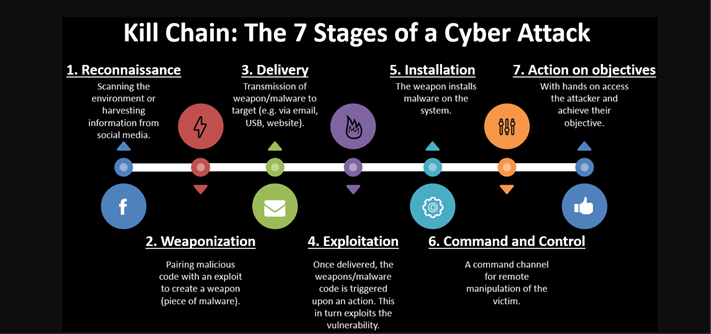
\includegraphics[width=350pt]{cyber_kill_chain}
    \caption{As 7 fases de um ataque cibernético}~\cite{kill-chain}
    \label{fig:chainimage}
\end{figure}

Também é importante mencionar as inúmeras organizações que ajudam e facilitam o combate aos ataques cibernéticos, sendo a mais destacada a MITRE ATT\&CK. \bigskip

A MITRE ATT\&CK é uma organização focada na obtenção de informações de ciberataques apenas por observação do que acontece no mundo digital. \ É conhecida por ter uma vasta base de dados de ataques com informações de quase todos os ataques que aconteceram. \par

\newpage

Além de identificar os problemas, também disponibiliza soluções para os mesmos, tudo isto sem qualquer custo tanto para uso pessoal como para uso empresarial. \ Isto obviamente reforça a ideia de colaboração, que é bastante importante no ramo da informática.

\subsubsection{Ordem de Volatilidade}
É muito importante ter em conta a ordem de volatilidade dos ficheiros criados por um sistema, pois devemos começar sempre pelos ficheiros que estão mais em contacto com o sistema em si(como ficheiros cache, RAM, etc.). \ A ordem por base no tempo em que estão disponíveis e acessíveis é, respetivamente:
\begin{enumerate}
    \item Ficheiros cache
    \item Memória(RAM)
    \item Estado da rede
    \item Processos ativos
    \item Armazenamento
    \item Backups / Cópias de Segurança
    \item DVD's ou impressões
\end{enumerate}

Esta ordem é importante pelo facto de ao examinar um sistema, é preciso ter precisão para encontrar a origem do problema, e na maioria dos casos essas evidências estão na memória gerada pelo sistema no instante em que ocorre o ataque, sendo esse o foco principal de um investigador.

%%%%%%%%%%%%%%%%%%%%%%%%%%%%%%%%%%%%%%%%%%%%%

\section{Análise de evidências}
\label{sec:analise-de-evidencias}
A análise de evidências é muito importante para o desenvolvimento de métodos eficazes para combate a malwares, pois permite-nos examinar máquinas que foram afetadas por qualquer tipo de ameaça. \ Estas podem ser, por exemplo:
\begin{itemize}
    \item Malware
    \item Spyware
    \item Trojans
    \item Ransomware
\end{itemize}

\subsection{Vulnerabilidades e como combatê-las}
\label{subsec:vulnerabilidades-e-como-combate-las}
Quando se fala em vulnerabilidades, refere-se a uma possível falha num sistema que, a partir da mesma, pode ser comprometido o sistema, o utilizador ou uma empresa. \ Deve ser encarada como algo de alta prioridade, e deve ser resolvida o quão antes possível, antes que ocorra algo inesperado. \ Por este motivo deve sempre existir a identificação, análise e retificação de vulnerabilidades. \bigskip

Como forma de ajuda a combater vulnerabilidades, existem vários websites com as vulnerabilidades mais comuns, e todas as informações necessárias para poder saber a sua origem e como combatê-las.

\subsubsection{\ac{cve}}
 A~\ac{cve} \href{https://www.cve.org/}{(website)} e um projeto da MITRE, cujo intuito é identificar, definir e catalogar as várias vulnerabilidades que existem no mundo digital. \ Estas ameaças são sempre publicadas por parceiros da própria \ac{cve}, obtendo assim uma consistência nas descrições das vulnerabilidades, para quem desejar explorar múltiplas vulnerabilidades e não ter muitos conflitos com as explicações das mesmas.

\subsubsection{\ac{cvss}}
A \ac{cvss} \href{https://www.first.org/cvss/}{(website)} é um sistema que atribui a cada vulnerabilidade um grau de gravidade. \ Este é classificado\footnote{Fonte: \url{https://nvd.nist.gov/vuln-metrics/cvss}} do seguinte modo:

\begin{table}[htp]
    \begin{center}
    \begin{tabular}{|l||c||r|}
        \hline
            Severity   & Base Score Range \\   \hline\hline
            None       & 0.0          \\       \hline
            Low        & 0.1 - 3.9    \\       \hline
            Medium     & 4.0 - 6.9    \\       \hline
            High       & 7.0 - 8.9    \\       \hline
            Critical   & 9.0 - 10.0   \\       \hline
    \end{tabular}
    \end{center}
    \caption{CVSS Score}
    \centerline{A tabela acima representa os graus de gravidade na classificação \ac{cvss}}
    \label{tab:cvss}
\end{table}

Apenas são usados valores definitivos, que significa que não vai existir mudança de valores para uma vulnerabilidade. \ Daí surgir a importância de uma calculadora capaz de medir com precisão o grau de gravidade de uma vulnerabilidade. \ Se a mesma se agravar, é criado um novo catálogo com a nova ameaça.

\subsubsection{\ac{cwe}}
A \ac{cwe} \href{https://cwe.mitre.org/}{(website)} é outro projeto da MITRE, que lista todos os tipos de fraquezas de software e hardware comuns. \ Uma fraqueza é uma condição num software, hardware, firmware ou serviço que pode vir a introduzir uma vulnerabilidade a partir delas. \par
O grande objetivo da \ac{cwe} é parar as vulnerabilidades na sua raíz, educando qualquer pessoa que trabalha no ramo da informática, de modo a evitar erros comuns e contribuir para um espaço mais seguro numa empresa.

\subsubsection{\ac{owasp}}
O \ac{owasp} \href{https://owasp.org/}{(website)} é uma fundação open-source com o intuito de melhorar a segurança de softwares no geral, ensinando pessoas pelo mundo todo para existir uma web mais segura. \bigskip

Dentro desta fundação, foi criada um projeto bastante importante no mundo cibernético, o OWASP Top Ten~\cite{top-10}. \ Este projeto consiste em, no final de cada ano, organizar um top 10 das ameaças mais comuns nesse mesmo ano. \ É feito sempre uma comparação com anos anteriores para verificar as mudanças e melhorias que aconteceram. \ Ao ser realizada a comparação, consegue-se saber se houve melhorias face ao combate de vulnerabilidades anteriores, as novas vulnerabilidades introduzidas e uma breve explicação de cada uma delas. \bigskip

No seguinte esquema~\footnote{Fonte: \url{https://owasp.org/www-project-top-ten/}}, está representada a comparação das vulnerabilidades do ano 2017, e do ano 2021:

\begin{figure}[h]
    \centering
    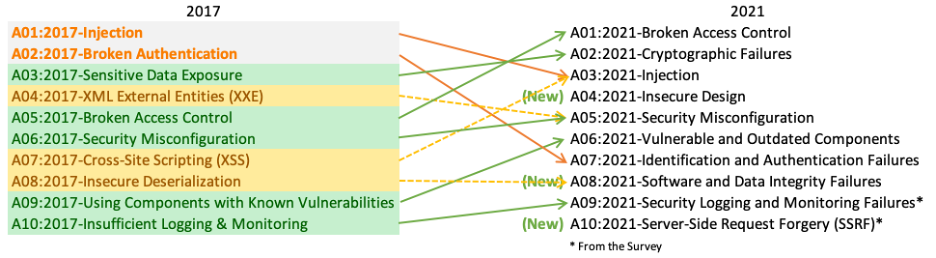
\includegraphics[width=350pt]{top10-2021}
    \caption{Comparação das ameaças mais comuns entre 2017 e 2021}
    \label{fig:top10-2021}
\end{figure}

%%%%%%%%%%%%%%%%%%%%%%%%%%%%%%%%%%%%%%%%%%%

\subsection{Softwares usados para análises}
\label{subsec:softwares-usados-para-analises}
Para poder examinar e tirar conclusões de anomalias nos sistemas, é necessário utilizar software dedicado para este tipo de problemas. \ Os softwares mais utilizados são o~\nameref{subsubsec:autopsy}, o~\autoref{subsubsec:owasp-zap}, e o~\nameref{subsubsec:docker}. \par
Também é importante referir que para examinar discos e outras unidades de memória, é necessário usar uma máquina virtual~\nameref{subsubsec:kali}. \par

\subsubsection{Kali}
\label{subsubsec:kali}
O Kali é um sistema operativo Linux de base Debian. \ É usada especificamente para análise de vulnerabilidades, invasão de redes, entre outros fins de forense. \  No \href{https://www.kali.org/get-kali/}{site oficial} existem várias opções de download do Kali. \ Uma das mais utilizadas para análise de máquinas é a Live Boot. \bigskip

A Live Boot consiste num sistema operativo temporário e inalterável, ou seja, ao reiniciar ou desligar, volta às definições default. \ Como não se pode fazer alterações definitivas na máquina, ela tem de estar pré-definida com os programas necessários para qualquer tipo de análise. \ Por ser um sistema inalterável, tem a vantagem de ser possível mexer nas evidências sem correr o risco de alterar as mesmas, algo que invalidaria automaticamente as provas. \par
Por ser um sistema de base Linux, grande parte dos sistemas de ficheiros são acessíveis, algo que não é possível num sistema Windows. \bigskip

Existe também a possibilidade de uma máquina virtual que use um disco virtual, que significa que guarda todas as alteracções como um computador faria. \ Este tipo de máquina é usada para explorar vulnerabilidades, por exemplo, em websites. \par
Estas ferramentas devem ser usadas explicitamente com o consentimento total da vítima, sendo estritamente proibido realizar um ataque não autorizado a qualquer empresa ou indivíduo. \ São apenas ferramentas para fundos de educação.


\subsubsection{Autopsy}
\label{subsubsec:autopsy}
O Autopsy é uma aplicação open-source que é capaz de analisar quase todos os tipos de discos, e foi escrita em Java. \ Esta usa plugins feitos pela comunidade para uma experiência customizável para cada utilizador, permitindo assim uma livre escolha dependendo das necessidades de cada pessoa. \par
Esta aplicação é focada em vários campos, como, por exemplo:
\begin{itemize}
    \item Pesquisas em Universidades/Academias
    \item Investigações em empresas
    \item Governo e Órgãos militares
    \item Investigações na polícia
\end{itemize}
A grande vantagem de usar o Autopsy ao invés de usar um sistema Kali por Live Boot, é que pode-se analisar unidades de disco diretamente a partir do sistema operativo principal, aumentando significamente a performance da análise, pois não se usa uma pen ou uma máquina virtual para usar o sistema operativo.

% TODO : finish owasp-zap and docker

\subsubsection{\ac{owasp-zap}}
\label{subsubsec:owasp-zap}
A \ac{owasp-zap} é uma aplicação open-source desenvolvida pela \ac{owasp}, com o objetivo de explorar vulnerabilidades num website. \ O programa vem com inúmeras ferramentas de Penetration Testing, para detetar o máximo de vulnerabiliades possíveis. \par
Esta aplicação tem como vantagens:
\begin{itemize}
    \item Ser reutilizável, sendo capaz de guardar reports
    \item Bom para iniciantes
    \item É grátis
\end{itemize}
Por outro lado, não é a ferramenta mais prática de usar em empresas, pelo facto de ser open-source e não ter tanta privacidade como outras ferramentas pagas. \par
É recomendado pela \ac{owasp} o uso desta aplicação juntamente com o~\nameref{subsubsec:docker}, para a automatização das ferramentas existentes no programa. \bigskip
Também é importante referir o projeto Juice Shop, que consiste numa aplicação escrita em JavaScript e que simula uma loja genérica de vários produtos, que contém uma série de vulnerabilidades. \par
É aconselhado usar a imagem deste projeto no Docker, para a exploração dos erros ser efetuada localmente e eficientemente. \ Estes erros têm vários graus de dificuldade de serem explorados, e à medida que se descobre os erros, eles vão sendo guardados num ficheiro log que contém o que já foi descoberto pelo untilizador.

\subsubsection{Docker}
\label{subsubsec:docker}
O Docker é um programa usado para desenvolver, enviar e correr aplicações. \ Desta forma, pode-se criar vários containers para correr ou enviar qualquer tipo de aplicação num espaço isolado. \ Tem a vantagem de poder ter várias aplicações a correr localmente no mesmo sistema sem consumir muito hardware, que é um grande benefício na área da cibersegurança, pois é usado vários programas ao mesmo tempo.

\begin{figure}
    \centering
    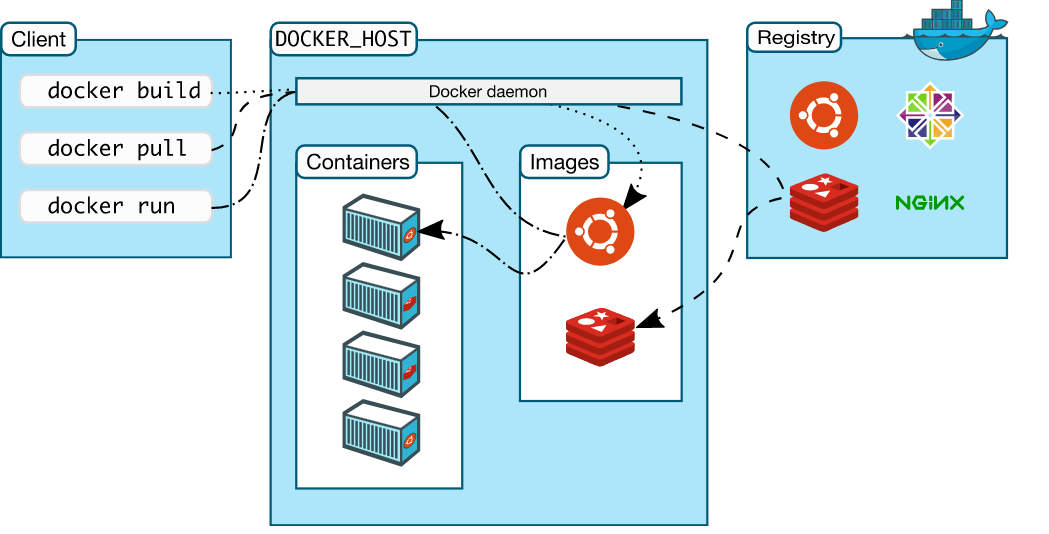
\includegraphics[width=350pt]{docker-scheme}
    \caption{Esquema que representa o funcionamento do Docker}
    \label{fig:docker-scheme}
\end{figure}

Os containers são feitos e funcionam em base de imagens, semelhante a um sistema operativo. \ Estas são normalmente imagens de outras imagens, apenas com algumas modificações feitas. \bigskip

Uma imagem bastante conhecida neste campo é a imagem do Juice Shop, um projeto referido na \autoref{subsubsec:owasp-zap} \ Com o Docker e a imagem deste projeto, podemos criar um container que vai correr o site, localmente. \ A grande vantagem de correr ficheiros localmente é que pode-se fazer os testes sem qualquer problema, é possível fazer certos tipos de ataque que na Internet seriam considerados ilegais mas que são, sem dúvida alguma, cruciais para o bom funcionamento de um website.

\chapter{Soluções de segurança}
\label{ch:solucoes-de-seguranca}

\chapter{Conclusões}
\label{ch:conclusao}
Apresenta conclusões.

\chapter*{Contribuições dos autores}
Cada autor contribuiu igualmente para o produto final do trabalho, sendo justamente atribuído a nota de 50\% a cada um. \\
O autor \ac{rg} realizou o capítulo de Vulnerabilidades completo. \\
O autor \ac{tg} realizou o capítulo de Cibersegurança no geral e Soluções de segurança.

\vspace{10pt}
\textbf{Indicar a percentagem de contribuição de cada autor.}\\

\ac{rg}, \ac{tg} : 50\%, 50\%\\

%%%%%%%%%%%%%%%%%%%%%%%%%%%%%%%%%

\chapter*{Acrónimos}
\begin{acronym}
    \acro{api}[API]{Application Programming Interface}
    \acro{ddos}[DDOS]{Distributed denial-of-service}
    \acro{http}[HTTP]{Hypertext Transfer Protocol}
    \acro{iot}[IOT]{Internet of Things}
    \acro{leci}[LECI]{Licenciatura em Engenharia de Computadores e Informática}
    \acro{rg}[RG]{Rúben Gomes}
    \acro{rgpd}[RGPD]{Regulamento Geral sobre a Proteção de Dados}
    \acro{tg}[TG]{Tiago Garcia}
    \acro{ua}[UA]{Universidade de Aveiro}
    \acro{dfi}[DFI]{Digital Forensic Investigation}
    \acro{cirts}[CIRTs]{Computer Incident Response Teams}
    \acro{certs}[CERTs]{Computer Emergency Response Teams}
    \acro{cve}[CVE]{Common Vulnerabilities and Exposures}
    \acro{cvss}[CVSS]{Common Vulnerability Scoring System}
    \acro{cwe}[CWE]{Common Weakness and Enumeration}
    \acro{owasp}[OWASP]{Open Web Application Security Project}
    \acro{owasp-zap}[OWASP-ZAP]{OWASP - Zed Attack Proxy}
\end{acronym}


%%%%%%%%%%%%%%%%%%%%%%%%%%%%%%%%%
\printbibliography

\end{document}
